\chapter[Test e Performance]{Test e Performance}

Una gran parte della letteratura descritta nel secondo capitolo giunge a una conclusione importante sulle operazioni di analisi dei gestori dinamici di memoria: per valutare un algoritmo di allocazione, è necessario osservarne il comportamento e la risposta del sistema a un contesto realistico. Ciò può avvenire solamente laddove le tracce adoperate per condurre i \textit{benchmark} siano vicine alle allocazioni realmente compiute da programmi reali, che sono presi come esempio (esistono \textit{utilities} che permettono di registrare le richieste, in modo da poterle usare a questo scopo).

Quando le tracce sono casualmente generate, il risultato finale ci dice ben poco sulle capacità effettive delle politiche di assegnazione. Le richieste prodotte da un generatore probabilistico possono anche ispirarsi ad un modello di comportamento, ma questo non è sufficiente: riprodurre le complesse interazioni tra allocazioni e deallocazioni di memoria è molto difficile, poiché queste ultime sono poco comprese e differiscono grandemente tra tipologie di applicazione. Il comportamento a fasi dei programmi dà vita a fenomeni di interconnessione sistematica che sono per la maggior parte ignorati.

Nel 1998, Wilson e Johnston approfondiscono i risultati del procedente \textit{paper} sull’allocazione dinamica di memoria indagando il comportamento di diversi noti programmi scritti in C e C++. Nell’articolo \textit{``The Memory Fragmentation Problem: Solved?''}\cite{wilson1998} gli autori tentano di dimostrare come la frammentazione può essere evitata laddove sia scelta con attenzione una politica di allocazione appropriata a prescindere dall’implementazione: questi risultati sono significativi perché suggeriscono che sia opportuno spostare la concentrazione di energie dal ridurre la frammentazione e dirigerle piuttosto nella direzione corrispondente a implementazioni più efficenti.

\begin{quote}
``This substantially strengthens our previous results showing that the memory fragmentation problem has generally been misunderstood, and that good allocator policies can provide good memory usage for most programs. The new results indicate that for most programs, excellent allocator policies are readily available, and efficiency of implementation is the major challenge.''

\begin{center}
[...]
\end{center}

``If these results hold up to further study with additional programs, we arrive at the conclusion that the fragmentation problem is a problem of recognizing that good allocation policies already exist, and have inexpensive implementations. For most programs, the problem of simple overheads is more significant than the problem of fragmentation itself.''
\end{quote} 

Il programma è stato sottoposto anche ad analisi attraverso \textit{valgrind}, il popolare programma di \textit{debugging} e \textit{memory analysis}, in particolare adoperando i \textit{tool} \textit{memcheck, massif} e \textit{cachegrind}. Questi strumenti sono stati fondamentali per comprendere in primo luogo se il programma accedesse alla memoria come previsto, e secondariamente per comprendere dove si trovassero le ostruzioni e i punti critici che causavano perdita di efficienza. Sfortunatamente, l'analisi della memoria richiesta al sistema operativo attraverso le operazioni di \texttt{mmap} non è altrettanto immediata quanto invece per quella ottenuta via \texttt{malloc}. Nonostante queste difficoltà, i risultati che siamo stati in grado di ottenere sono soddisfacenti in una prima fase esplorativa.

\section{Test delle funzionalità}

I test delle funzionalità si concentrano unicamente sulla correttezza del codice: verificano che le funzioni rispondano correttamente a parametri sbagliati o richieste inappropriate. Definendo la flag \texttt{DEBUG} a tempo di compilazione abbiamo accesso a maggiori informazioni sugli errori e sulle loro cause. 

\subsection{SlabAllocator}
\begin{table}[H]
\centering
\begin{tabularx}{\textwidth}{|l|X|}
\hline
\textbf{Nome del Test} & \textbf{Descrizione} \\
\hline
\texttt{test\_invalid\_init} & Verifica che l'allocatore gestisca correttamente parametri di inizializzazione non validi (es. dimensione zero o numero massimo di slab non valido). \\
\hline
\texttt{test\_create\_destroy} & Controlla che la creazione e distruzione di uno slab avvengano correttamente, senza memory leak o errori. \\
\hline
\texttt{test\_alloc\_pattern} & Testa il comportamento dell'allocatore con un pattern di allocazioni e deallocazioni ripetute per verificare la correttezza della gestione della memoria. \\
\hline
\texttt{test\_exhaustion} & Verifica il comportamento quando lo slab è pieno (es. ritorno di NULL o gestione degli errori quando non c'è più memoria disponibile). \\
\hline
\texttt{test\_invalid\_free} & Controlla come l'allocatore gestisce la deallocazione di puntatori non validi (es. NULL o indirizzi non allocati). \\
\hline
\end{tabularx}
\caption{Test funzionali per SlabAllocator}
\end{table}

I test per lo SlabAllocator sono generalmente semplici in natura: poiché la grandezza della richiesta non varia e la lista da gestire è singola, gli unici punti di difficoltà sono la creazione con parametri invalidi o il rilascio di puntatori incorretti.


\subsection{BuddyAllocator e BitmapBuddyAllocator}
\begin{table}[H]
\centering
\begin{tabularx}{\textwidth}{|l|X|}
\hline
\textbf{Nome del Test} & \textbf{Descrizione} \\
\hline
\texttt{test\_invalid\_init} & Verifica che l'allocatore gestisca correttamente inizializzazioni non valide (es. dimensione zero, parametri NULL, o valori non supportati). \\
\hline
\texttt{test\_create\_destroy} & Testa la corretta creazione e distruzione di un allocatore, assicurandosi che non ci siano memory leak o corruzione dei dati. \\
\hline
\texttt{test\_single\_allocation} & Verifica che l'allocatore possa rispondere correttamente ad allocazioni invalide e gestire correttamente una singola allocazione. \\
\hline
\texttt{test\_multiple\_allocation} & Controlla il comportamento dell'allocatore quando vengono effettuate più allocazioni consecutive, assicurandosi che tutte abbiano successo e non si sovrappongano. \\
\hline
\texttt{test\_varied\_sizes} & Testa l'allocazione di blocchi di dimensioni diverse per verificare che l'allocatore gestisca correttamente richieste eterogenee. \\
\hline
\texttt{test\_buddy\_merging} & Verifica che, dopo una serie di allocazioni e deallocazioni, l'allocatore riesca a fondere correttamente i blocchi liberi adiacenti (buddy merging) per evitare frammentazione. \\
\hline
\texttt{test\_invalid\_reference} & Controlla come l'allocatore gestisce tentativi di deallocazione di riferimenti non validi (es. NULL, doppio free, o puntatori non allocati). \\
\hline
\end{tabularx}
\caption{Test funzionali per BuddyAllocator e BitmapBuddyAllocator}
\end{table}

Gli allocatori che accettano richieste a taglia variabile presentano una complessità maggiore rispetto a quelli a taglia fissa, poiché devono gestire dinamicamente la suddivisione e la fusione dei blocchi di memoria per rispondere a richieste di dimensioni differenti. Questo comporta una maggiore probabilità di introdurre errori nella gestione della memoria come la perdita di riferimenti o la mancata fusione dei blocchi liberi (\textit{buddy merging}). I test svolgono un ruolo fondamentale nell'evidenziare anomalie e comportamenti indesiderati

Oltre ai test elencati, è utile prevedere casi limite e scenari di stress, come sequenze di allocazioni e deallocazioni ripetute con dimensioni variabili, tentativi di allocazione che saturano la memoria disponibile, e la verifica della corretta gestione di errori (ad esempio, \textit{double free} o allocazioni fuori dai limiti consentiti). Potrebbe essere positivo stabilire anche una serie standardizzata di messaggi d'errore per facilitare le operazioni di verifica: ciò non è stato fatto per mera mancanza di tempo. Un altro aspetto che è stato valutato di confermare consiste nello scrivere in tutta la memoria assegnata contemporaneamente e verificare che non ci sia corruzione dei dati. Funzioni sviluppate a questo scopo sono già esistenti nell'applicativo.

\section{Benchmark}
Poiché la nostra analisi si concentra principalmente sulla correttezza dell'implementazione, i test sopra delineati forniscono una prima conferma del nostro operato. Tuttavia, l'importanza della \textit{performance} dell'allocatore in diversi casi applicativi risulta essenziale per poter veramente trarre delle conclusioni a riguardo. 
Nel corso delle ricerche, l'articolo \textit{"Designing a Trace Format for Heap Allocation Events"}\cite{chilimbi2000} di T.Chilimbi et al ha fornito un'interessante base teorica per il \textit{parser} qui descritto. Tuttavia, il nostro vuole essere unicamente un prototipo di funzionamento al fine di svolgere analisi più profonde, e sicuramente fornisce ben poche delle capacità descritte nell'articolo o altrimenti rese disponibili da altri strumenti simili applicati nel campo.\footnotemark

\footnotetext{Alcuni di questi che menzioniamo per dovere di cronaca sono \texttt{perf, LTTng} e \texttt{ETW}. }

Per facilitare dunque l’analisi del comportamento degli allocatori in presenza di \textit{pattern} complessi di allocazione e deallocazione, è stata introdotta una funzionalità che consente di definire facilmente le sequenze di richieste di memoria tramite file di configurazione esterni, senza dover modificare o ricompilare il codice sorgente. In questo modo è possibile variare rapidamente i benchmark e testare diversi scenari. Il codice sorgente di questa funzionalità si trova nei moduli \texttt{benchmark} e \texttt{parse}.

Ciò è reso possibile dall’implementazione da parte di ogni allocatore dell’interfaccia \texttt{<Allocator>}. Poiché abbiamo a nostra disposizione i puntatori alle funzioni necessarie per svolgere tutte le operazioni, possiamo standardizzare il funzionamento delle classi dividendole in due categorie: allocatori a taglia fissa, che permettono di richiedere blocchi di grandezza prestabilita (e.g.\ \texttt{SlabAllocator}) e allocatori a taglia variabile, ossia le classi “figlie” di \texttt{VariableBlockAllocator}, le quali invece lasciano all’utente la scelta della dimensione dell’area di memoria richiesta (ossia \texttt{BuddyAllocator} e \texttt{BitmapBuddyAllocator}, nella nostra implementazione).

\begin{lstlisting}
  // template per allocatore a dimensione fissa
  void *FixedSizeAllocator_malloc(FixedSizeAllocator *a);
  void *FixedSizeAllocator_free(FixedSizeAllocator *a);
  // template per allocatore a dimensione variabile
  void *VariableSizeAllocator_malloc(VariableSizeAllocator *a, size_t size);
  void *VariableSizeAllocator_free(VariableSizeAllocator *a)
\end{lstlisting}

Il programma cerca all’interno della cartella \texttt{./benchmarks} file che abbiano l’estensione \texttt{.alloc}. Modificando il testo al loro interno si possono definire la tipologia di allocatore, i suoi parametri di inizializzazione e la sequenza di \texttt{malloc}/\texttt{free} da provare. I comandi sono terminati dal carattere ``a capo'' (\textbackslash n) e le componenti sono divise da una virgola. Comandi che sono preceduti dal carattere percentuale (\%) sono considerati commenti e ignorati.

Vediamo ora come descrivere la classe di allocatore da sottoporre al benchmark e le sue caratteristiche. La prima riga non preceduta da un segno percentuale deve avere necessariamente la seguente struttura: \texttt{i,<allocator class>} dove la classe può essere \texttt{slab}, \texttt{buddy} o \texttt{bitmap}. Il secondo comando informa il programma sui parametri di creazione: \texttt{p,<param1>,<param2>,\ldots}, il numero e il tipo dei quali varia in base alla classe scelta precedentemente.

\begin{table}[H]
\centering
\begin{tabularx}{\textwidth}{|X|X|X|X|}
\hline
\textbf{Allocatore} & \textbf{Dimensione} & \textbf{Parametro 1} & \textbf{Parametro 2} \\
\hline
Slab    & Fissa     & \texttt{slab\_size}   & \texttt{num\_slabs}   \\
\hline
Buddy   & Variabile & \texttt{memory\_size} & \texttt{max\_levels}  \\
\hline
Bitmap  & Variabile & \texttt{memory\_size} & \texttt{max\_levels}  \\
\hline
\end{tabularx}
\caption{Parametri di inizializzazione per ciascuna classe di allocatore}
\end{table}

Per allocare e liberare memoria, l’istruzione deve iniziare rispettivamente con ``a'' o ``f''. Il benchmark per tenere traccia delle allocazioni usa un array avente lunghezza pari al numero massimo possibile di frammenti di memoria che possono esistere contemporaneamente. Un possibile oggetto di rivalutazione potrebbe essere l'uso di strutture per immagazzinare simboli più complessi e tenere traccia degli indirizzi in modo più chiaro. Il comando \texttt{a,<index>} alloca memoria in una posizione specifica dell'array, mentre \texttt{f,<index>} la libera. Nel caso di allocatore a richiesta variabile, dopo l’index dell’array va specificato il numero di byte da allocare (con struttura \texttt{a,<index>,<size>}). 

È fondamentale non allocare più volte sullo stesso indice senza prima liberarlo, altrimenti si perderà il riferimento all'area di memoria e non sarà più possibile gestirla correttamente\footnotemark. Il programma esegue la sequenza di \textit{requests} e \textit{releases}, informa l'utente di eventuali errori e produce un informativa sul tempo richiesto a portare a termine il \textit{benchmark}: \texttt{elapsed\_seconds}, \texttt{user\_seconds} e \texttt{kernel\_seconds}. In più, produce un file di \texttt{.log} che contiene informazioni sulle singole istruzioni (in particolare, per i \texttt{VariableBlockAllocator}, inserisce anche lo stato della frammentazione interna ed esterna dell'allocatore a ogni istruzione).
L'analisi di queste informazioni fornisce alcune metriche aggiuntive sul comportamento dell'allocatore e sulla sua \textit{performance}.

\footnotetext{Il programma di benchmarking non esegue istruzioni che porterebbero alla perdita di un indirizzo e avverte se il benchmark termina senza deallocare tutti gli indirizzi.}

\subsection{Analisi dei pattern di allocazione}
La letteratura individua tre principali pattern di utilizzo della memoria che ricorrono nella maggior parte dei programmi. Questi modelli sono \textbf{rampe, picchi e plateau}\footnotemark. In particolare, Wilson et al. evidenziano come sia spesso possibile riconoscere, nel ciclo di vita di un programma, macrosequenze di allocazione e deallocazione che seguono questi modelli: inoltre, all'interno di tali pattern principali, possono emergere sottostrutture più piccole che ripetono dinamiche simili, riflettendo la complessità e la varietà dei comportamenti reali di gestione della memoria.

\footnotetext{Altri \textit{patterns} dell'uso di memoria possono essere incontrati, ma sono meno comuni: allo stesso modo, variazioni o combinazioni dei modelli qui citati sono spesso presenti.}

\begin{itemize}
  \item \textbf{\textit{Ramps}}: molti programmi accumulano determinate strutture dati in modo monotono. Ciò può essere dovuto al fatto che conservano un registro degli eventi o perché la strategia di risoluzione del problema richiede la costruzione di una rappresentazione di grandi dimensioni, dopo la quale è possibile trovare rapidamente una soluzione.\\
  \textit{Esempio:} parser di log che accumulano eventi in memoria, compilatori che costruiscono un AST, o applicazioni che caricano progressivamente dati da una sorgente esterna.

  \item \textbf{\textit{Peaks}}: molti programmi utilizzano la memoria in modo discontinuo, creando strutture dati relativamente grandi che vengono utilizzate per la durata di una particolare fase e poi la maggior parte o tutte le strutture dati viene scartata. Si noti che le strutture di dati “sopravvissute” sono probabilmente di tipo diverso, perché rappresentano i risultati di una fase, rispetto a valori intermedi che possono essere rappresentati in modo diverso. (Un \textit{peak} è come una \textit{ramp}, ma di durata più breve).\\
  \textit{Esempio:} algoritmi di \textit{sorting} che allocano buffer temporanei, elaborazione di immagini o video dove ogni frame richiede molta memoria temporanea, oppure fasi di calcolo numerico in cui vengono creati e poi distrutti grandi array temporanei.

  \item \textbf{\textit{Plateaus}}: molti programmi costruiscono rapidamente strutture dati e poi le utilizzano per lunghi periodi (spesso per quasi tutto il tempo di esecuzione del programma).\\
  \textit{Esempio:} web server che mantengono strutture dati per la gestione delle connessioni attive, database \textit{in-memory} che caricano dati all’avvio e li mantengono residenti, o giochi che caricano la mappa di gioco all’inizio e la usano per tutta la sessione.
\end{itemize}

\begin{figure}[H]
  \centering
  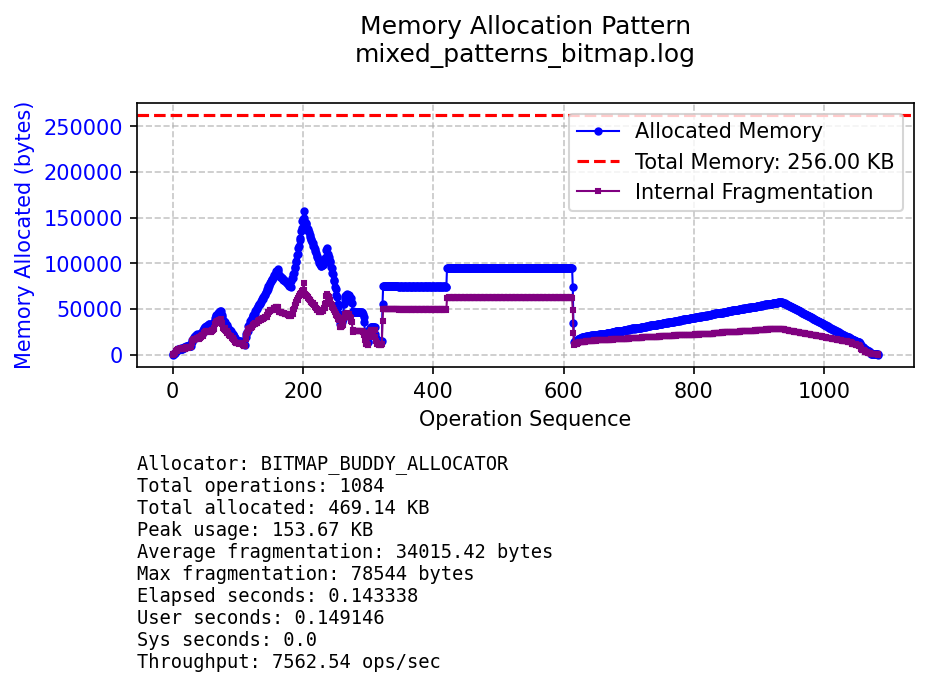
\includegraphics[width=1\textwidth]{graphs/mixed_patterns_bitmap.png}
  \caption{Comportamento del BitmapBuddyAllocator su un benchmark contenente in ordine, \textit{peaks, plateaus} e \textit{ramps}.}
  \label{fig:mixed_patterns_bitmap}
\end{figure}

\paragraph{Costo legato al logging.}
Utilizzando lo strumento da noi creato, siamo in grado di simulare questi \textit{pattern} e verificare il comportamento degli allocatori in loro presenza. Nel considerare i risultati ottenuti ricordiamo tuttavia che l'applicazione del \textit{profiling} comporta ovviamente un costo non trascurabile: i risultati successivamente riportati sono chiaramente influenzati dalle operazioni di \textit{logging} svolte dal programma. Sono state fatte numerose scelte nel tentativo di evitare costi eccessivi, ma sfortunatamente è impossibile analizzare gli allocatori così a fondo senza introdurre una misura di \textit{overhead}.

\subsection{Allocazioni sfavorevoli: frammentazione interna}

Come abbiamo menzionato precedentemente nella nostra analisi dell'implementazione degli allocatori che implementano un \textit{buddy system}, la possibilità di frammentazione interna molto elevata al punto da essere debilitante non è da trascurarsi. Adoperando lo strumento da noi creato per simulare un caso estremo, possiamo facilmente osservare dai grafici come determinate combinazioni di parametri di inizializzazione e richieste mal formulate possano rendere l'allocatore molto inefficace nel gestire la memoria a sua disposizione. Le linee rosse sul grafico rappresentano richieste che non è stato possibile soddisfare per via di frammentazione interna o esterna.
\begin{figure}[H]
  \centering
  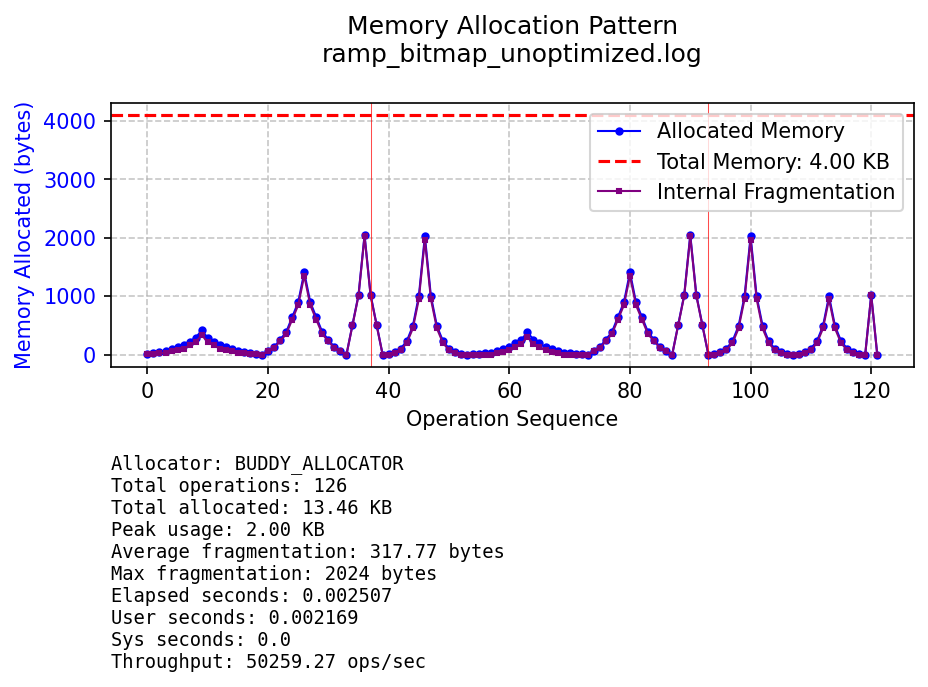
\includegraphics[width=0.9\textwidth]{graphs/ramp_bitmap_unoptimized.png}
  \caption{Sequenza di istruzioni che causano nel BuddyAllocator grande frammentazione interna. Notiamo che la quantità di memoria inutilizzabile è pari a quella allocata.}
  \label{fig:ramp_bitmap_unoptimized}
\end{figure}

Chiaramente, il caso riportato sopra risulta essere manipolato per esasperare il nostro punto. Non vi è alcun dubbio che sarebbe ben difficile incontrare in natura un pattern così sfortunato: tuttavia, bastano una serie di allocazioni mal concepite per rendere, soprattutto in corrispondenza di picchi di utilizzo, una cospicua parte della memoria inutilizzabile e pertanto riteniamo sia importante che il programmatore avveduto faccia uso di strumenti simili per comprendere il comportamento del proprio allocatore e, se necessario, apportare cambiamenti che lo rendano più adatto al proprio caso d'uso. Di seguito riportiamo altri due esempi di pattern in cui tuttavia è stata presa cura di minimizzare la frammentazione diminuendo le taglie degli oggetti allocati oppure, più semplicemente, aumentando di poco la dimensione dell'area di memoria che l'allocatore amministra.

\begin{figure}[H]
  \centering
  \begin{minipage}{0.5\textwidth}
    \centering
    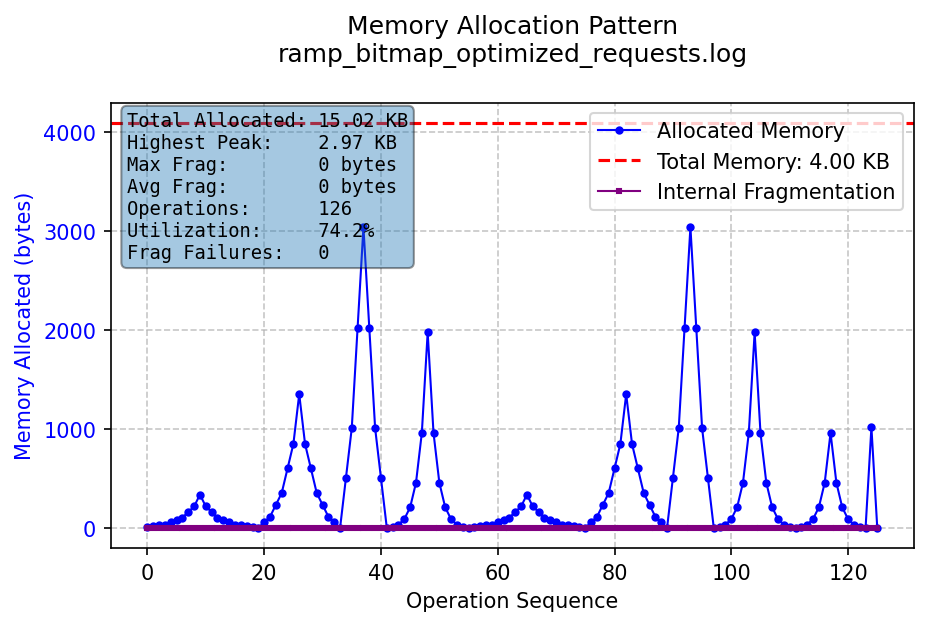
\includegraphics[width=0.95\textwidth]{graphs/ramp_bitmap_optimized_requests.png}
    \caption{Con richieste di dimensione leggermente minore, la frammentazione diventa irrilevante.}
    \label{fig:ramp_bitmap_optimized_requests}
  \end{minipage}\hfill
  \begin{minipage}{0.5\textwidth}
    \centering
    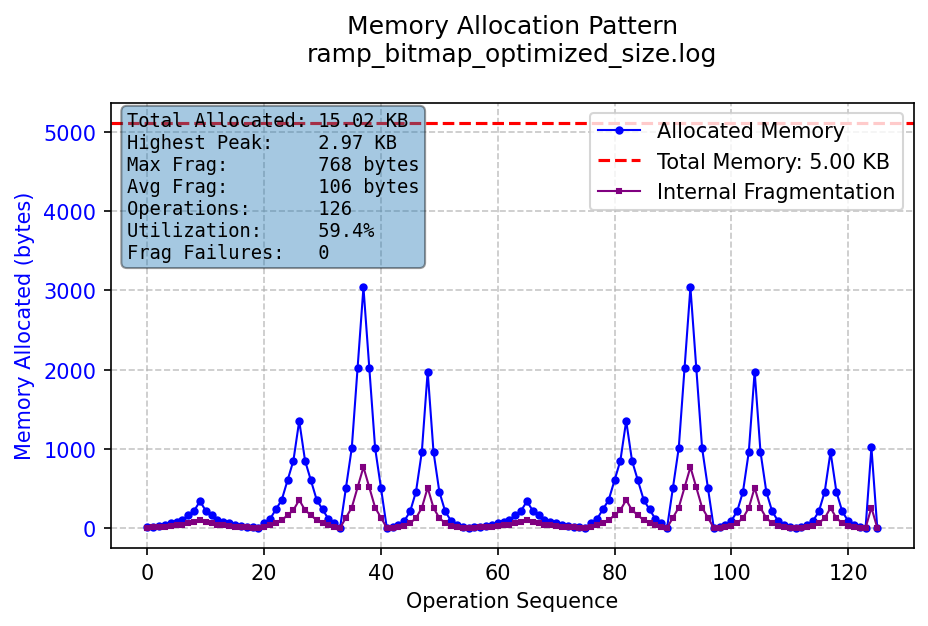
\includegraphics[width=0.95\textwidth]{graphs/ramp_bitmap_optimized_size.png}
    \caption{Allocando relativamente poca memoria in più, la frammentazione diminuisce sostanzialmente.}
    \label{fig:ramp_bitmap_optimized_size}
  \end{minipage}
\end{figure}


\subsection{LinkedList vs. Bitmap}

Sebbene esse siano quasi uguali in termini di frammentazione interna ed esterna (la politica di allocazione è difatti la medesima), la caratteristica che distigue il \texttt{BuddyAllocator} e il \texttt{BitmapBuddyAllocator} è la struttura dati adoperata per mantenere i riferimenti ai blocchi liberi, in quanto l'implementazione del primo adopera liste concatenate per rappresentare ogni livello. Questa scelta è stata fatta in quanto in ogni momento in ogni lista può essere presente un numero di elementi altamente variabile: la natura delle \textit{LinkedList} le rende quindi particolarmente adatte a svolgere questo ruolo. Ciononostante, nella prima iterazione questo allocatore è andato incontro a una problematica, di cui svolgiamo un'analisi nella sezione successiva.

Utilizzando lo strumento \texttt{cachegrind} e gli altri \textit{tool} compresi in \textit{valgrind}, abbiamo potuto svolgere un analisi più approfondita del comportamento del nostro programma, in particolare rilevando le differenze tra le due implementazioni del \textit{buddy system}. Il comportamento della cache dipende dalle caratteristiche del calcolatore. I test eseguiti di seguito sono stati svolti su un sistema avente le seguenti caratteristiche:
\begin{lstlisting}[language={}]
desc: I1 cache:   32768 B, 64 B, 8-way associative
desc: D1 cache:   32768 B, 64 B, 8-way associative
desc: LL cache:   6291456 B, 64 B, 12-way associative
\end{lstlisting}

Infine, i dati chiaramenti risentono della presenza delle infrastrutture di controllo e logging. Chiaramente gli accessi in memoria sono molti di più di quelli che avverrebbero in un'applicazione reale perché il programma sta salvando informazioni sullo stato. Poiché però lo "svantaggio" dato dalle risorse aggiuntive di cui sopra si applica in maniera uniforme a tutti i test, riteniamo non sia fuorviante condurre un'analisi relativa e comparata.

\subsubsection*{Prevenzione dei \textit{Double free}}
Un'analisi preliminare delle prestazioni del \texttt{BuddyAllocator} mostra che risulta significativamente più lento rispetto all'alternativa basata su bitmap. Questo dato conferma le aspettative teoriche di una maggiore complessità, ma l'entità della differenza osservata è superiore a quanto previsto e suggerisce la presenza di ulteriori fattori che penalizzano l'efficienza dell'implementazione.

\begin{lstlisting}
i,buddy
p,16276,10
I refs:        13,289,525
I1  misses:         2,910
LLi misses:         2,459
I1  miss rate:       0.02%
LLi miss rate:       0.02%

D refs:         8,944,880  (7,197,682 rd   + 1,747,198 wr)
D1  misses:     1,229,603  (1,217,474 rd   +    12,129 wr)
LLd misses:         6,545  (    1,608 rd   +     4,937 wr)
D1  miss rate:       13.7% (     16.9%     +       0.7%  )
LLd miss rate:        0.1% (      0.0%     +       0.3%  )

LL refs:        1,232,513  (1,220,384 rd   +    12,129 wr)
LL misses:          9,004  (    4,067 rd   +     4,937 wr)
LL miss rate:         0.0% (      0.0%     +       0.3%  )
\end{lstlisting}
\begin{itemize}
  \item \textbf{I refs}: Fetch istruzioni; \textbf{I1/LLi misses}: Mancati accessi cache istruzioni (primo/ultimo livello); \textbf{I1/LLi miss rate}: Percentuale miss cache istruzioni.
  \item \textbf{D refs}: Accessi dati (letture/scritture); \textbf{D1/LLd misses}: Mancati accessi cache dati (primo/ultimo livello, letture/scritture); \textbf{D1/LLd miss rate}: Percentuale miss cache dati.
  \item \textbf{LL refs}: Accessi totali cache ultimo livello; \textbf{LL misses}: Mancati accessi totali; \textbf{LL miss rate}: Percentuale miss cache ultimo livello.
\end{itemize}

Come vediamo facilmente, il programma così formulato ha un altissimo numero di istruzioni che accedono alla memoria, e da un'analisi più approfondita scopriamo che ciò avviene per la maggior parte proprio all'interno della funzione \texttt{list\_find}. Questa funzione è chiamata unicamente all'interno dello \texttt{SlabAllocator}, in particolare come parte delle verifiche di correttezza del programma. 

\begin{table}[H]
\centering
\begin{tabularx}{\textwidth}{|X|c|c|c|}
\hline
\textbf{Funzione} & \textbf{Ir (\%)} & \textbf{Dr (\%)} & \textbf{Dw (\%)} \\
\hline
\texttt{list\_find} & 9,633,626 (72.49\%) & 6,018,037 (83.61\%) & 1,205,430 (68.99\%) \\
\hline
\end{tabularx}
\caption{Profilazione della funzione \texttt{list\_find} in \texttt{double\_linked\_list.c}: Ir = \textit{Istruction, read}, Dr = \textit{Data, read}, Dw = \textit{Data, write}.}
\end{table}

All'interno del \texttt{BuddyAllocator} sono presenti due \texttt{SlabAllocator} per uso interno. Uno di essi in particolare, \texttt{node\_allocator}, si occupa di gestire la memoria necessaria per mantenere i \texttt{BuddyNode}: essi contengono le informazioni sui \textit{buddies} e sono quindi indispensabili. Quando la memoria viene rilasciata nel \texttt{BuddyAllocator}, se due \textit{buddies} sono liberi e pertanto riunificati, i \texttt{BuddyNodes} contenenti le informazioni su di essi vengono a loro volta riconsegnati alla \textit{free list} dello \texttt{SlabAllocator}. Quando esso riprende possesso di uno \textit{slab}, si assicura che non sia stato precedentemente rilasciato (evitando l'errore noto come \textit{double free}). Questa verifica può essere fatta attraverso la scansione della lista contenente tutti gli slab liberi, che è molto costosa poiché il costo è lineare al numero degli stessi. 

La nostra implementazione, per mantenere le informazioni necessarie per costruire i log, finisce per esacerbare il problema: il numero di slab nella lista è dato da $2^{L+1}$\footnotemark, dove $L$ rappresenta il numero di livelli dell'allocatore, in quanto, partizionando la memoria, dobbiamo tenere un riferimento non solo ai \textit{buddies}, ma anche ai genitori. In fase di sviluppo abbiamo menzionato che sarebbe possibile ottenere le informazioni del genitore dinamicamente, ma avevamo scelto di fare altrimenti per semplificare la raccolta di informazioni. Il numero di istruzioni che accedono alla memoria diventa quindi altissimo: l'efficienza ne risente a causa dell'elevato numero di \textit{data cache miss}.

\footnotetext{Uno per ogni nodo di un albero binario completo.}

\begin{lstlisting}
  // Check if node is already in free list using list_find
  if (list_find(slab->free_list, &slab_node->node)) {
      #ifdef DEBUG
      printf(RED "ERROR: Failed to free: slab node already in free list!\n" RESET);
      #endif
      return NULL;
  }
\end{lstlisting}

Per evitare la scansione lineare, la soluzione applicata è l'utilizzo di una flag all'interno di \texttt{SlabNode}, \texttt{bool in\_free\_list}, che ci permette di verificare più rapidamente se il blocco sia stato già liberato e quindi aggiunto alla \texttt{free list}. Questo check tuttavia è molto meno sicuro, e se il dato venisse corrotto permetterebbe il \textit{double free} di uno slab, che potrebbe dunque essere restituito due volte come risultato di una richiesta di memoria. 

\subsubsection{Efficienza della cache}

A seguito dell'ottimizzazione vista precedentemente, il comportamento dell'implementazione di \texttt{BuddyAllocator} che adopera le \textit{linked list} produce risultati molto migliori. Il numero di istruzioni è ridotto significativamente, così come la quantità di \textit{data reference} e conseguentemente dei cache miss. Viene tuttavia pagato un caro prezzo in termini di memoria da allocare per gestire la struttura ad albero: in particolare, un allocatore caratterizzato da un numero elevato di livelli richiede che sia adoperata moltissima memoria per gestire lo \texttt{SlabAllocator} al suo interno. Questo tuttavia si traduce in risultati molto positivi da punto di vista dell'efficenza temporale delle operazioni di allocazione e deallocazione, che avvengono molto velocemente. Verifichiamo \textit{throughput}, in base alla sequenza scelta, nell'ordine delle centinaia di migliaia di operazioni al secondo. 

Contemporaneamente però, alle preoccupazioni sulla quantità di memoria necessaria all'allocatore se ne aggiungono altre sulla non località della cache. La memoria gestita e quella usata a scopi organizzativi sono diverse, e quindi non abbiamo nessuna assicurazione sul comportamento del buffer: questo comporta maggiore imprevedibilità nella previsione delle \textit{performance} dell'allocatore. Ricordiamo infatti che il nostro benchmark non accede alla memoria allocata: pertanto il quadro a nostra disposizione non è completo e sicuramente in casi d'uso reali l'efficienza della cache che si trovi allo stesso tempo a gestire le richieste di accesso ai dati da parte dell'utente si comporterebbe in modo assai meno efficiente, in quanto verrebbero anche caricate nella memoria temporanea linee di cache in ordine per noi imprevedibile. 

\begin{lstlisting}[language={}]
i,buddy
p,16276,10

I refs:        3,652,823
I1  misses:        2,913
LLi misses:        2,463
I1  miss rate:      0.08%
LLi miss rate:      0.07%

D refs:        1,719,901  (1,178,874 rd   + 541,027 wr)
D1  misses:        7,915  (    2,430 rd   +   5,485 wr)
LLd misses:        6,545  (    1,608 rd   +   4,937 wr)
D1  miss rate:       0.5% (      0.2%     +     1.0%  )
LLd miss rate:       0.4% (      0.1%     +     0.9%  )

LL refs:          10,828  (    5,343 rd   +   5,485 wr)
LL misses:         9,008  (    4,071 rd   +   4,937 wr)
LL miss rate:        0.2% (      0.1%     +     0.9%  )
\end{lstlisting}

In contrasto con i risultati ottenuti per l'implementazione originale del \textit{buddy system}, la classe \texttt{BitmapBuddyAllocator} presenta risultati ben diversi. Il numero delle istruzioni ritorna ad essere molto elevato: ciò è dovuto alla natura ricorsiva delle funzioni di manipolazione della bitmap, che deve essere aggiornata quando cambia lo stato. Non escludiamo che sia possibile, forse dedicando più risorse per mantenere lo stato della memoria gestita, evitare questo numero così alto. Dal punto di vista della rapidità, il programma ne risulta sicuramente rallentato: tuttavia, la località della cache è molto migliore. Il numero di miss è irrisorio e sappiamo anche che la quantità di memoria necessaria per immagazzinare le informazioni è minore. La bitmap infatti è compatta e può essere più facilmente immagazzinata nella memoria intermedia. 

\begin{lstlisting}[language={}]
i,bitmap
p,16276,10

I refs:        14,221,610
I1  misses:         2,790
LLi misses:         2,460
I1  miss rate:       0.02%
LLi miss rate:       0.02%

D refs:         7,089,558  (4,813,930 rd   + 2,275,628 wr)
D1  misses:         4,567  (    2,269 rd   +     2,298 wr)
LLd misses:         3,405  (    1,616 rd   +     1,789 wr)
D1  miss rate:        0.1% (      0.0%     +       0.1%  )
LLd miss rate:        0.0% (      0.0%     +       0.1%  )

LL refs:            7,357  (    5,059 rd   +     2,298 wr)
LL misses:          5,865  (    4,076 rd   +     1,789 wr)
LL miss rate:         0.0% (      0.0%     +       0.1%  )
\end{lstlisting}

I risultati ottenuti ci forniscono le seguenti linee guida:

Se il tempo è critico e la quantità di memoria non è un fattore, BuddyAllocator fornisce un throughput ben maggiore e, con alcune ottimizzazioni ulteriori, potrebbe risultare la soluzione migliore per buddy system dalla scarsa profondità, in quanto il numero dei nodi cresce con il suo quadrato. 
Ad esempio, in un sistema operativo o in un hypervisor dove si devono gestire moltissime allocazioni e deallocazioni al secondo (come nel caso di un server di rete o un sistema real-time), l'elevata velocità di risposta del BuddyAllocator è cruciale e giustifica il maggiore uso di memoria.

Nei casi dove la memoria scarseggia ed è essenziale sfruttare al massimo l'efficacia della cache, il BitmapBuddyAllocator splende per località e semplicità. Le sue caratteristiche lo rendono più adatto quando è necessario avere performance stabili e prevedibili anche sotto carico realistico.
In ambienti embedded o su dispositivi IoT dove la RAM è limitata (es. microcontrollori con pochi KB/MB di memoria), oppure in sistemi mobile o edge computing, l'uso efficiente della cache e la ridotta impronta della bitmap sono essenziali per garantire affidabilità e reattività.

\paragraph{Considerazioni sulla thread safety.}
Se si richiedesse di integrare l'implementazione degli allocatori in modo che essi siano \textit{thread safe}, i fattori da considerare aumenterebbero ulteriormente. La gestione concorrente delle liste concatenate nel \texttt{BuddyAllocator} richiederebbe l'uso di meccanismi di sincronizzazione più complessi (ad esempio, mutex o lock per ogni lista), aumentando il rischio di contese e rallentando le operazioni in presenza di molti thread. Al contrario, la struttura compatta e lineare della bitmap nel \texttt{BitmapBuddyAllocator} si presta meglio a implementazioni thread safe, poiché è più semplice proteggere sezioni critiche e, in alcuni casi, è possibile sfruttare operazioni atomiche su bit per ridurre l'overhead della sincronizzazione. Pertanto, in scenari multithreaded, il \texttt{BitmapBuddyAllocator} risulta generalmente preferibile per la maggiore scalabilità e semplicità nella gestione della concorrenza.

\pagebreak

\subsection{Esempi di file \texttt{.alloc}}
\begin{lstlisting}[language={}]
% Tipo di allocatore (Slab)
i,slab         
% Parametri: slab_size=64, num_slabs=16
p,64,16        
% Alloca un blocco nell'indice 0
a,0            
% Alloca un blocco nell'indice 1
a,1            
% Libera il blocco nell'indice 0
f,0      
\end{lstlisting}      

Il programma di benchmarking in questo caso avvertirà l'utente che un blocco di memoria non è stato rilasciato entro la conclusione della sequenza (il blocco all'indice 1). Poiché in questo caso abbiamo inizializzato un \texttt{FixedBlockAllocator}, le richieste non esplicitano una quantità di byte. Una possibilità che in questo momento non è sfruttata consiste nel comunicare agli allocatori a dimensione fissa (in questo caso allo \texttt{SlabAllocator}) la dimensione dell'oggetto per poter immagazzinare informazioni sulla sua frammentazione interna. Supponendo però che il programmatore non adoperi lo stesso allocatore per oggetti diversi (che corrisponde al più comune caso d'uso), questa metrica sarebbe poco incisiva e rilevante. Pertanto per semplicità non è stata adottata.

\begin{lstlisting}[language={}]
% Benchmark per allocatore variabile
i,buddy
% memory_size=1024, max_levels=5
p,1024,5       
% L0->1024B, L1->512B, L2->256B, L3->128B, L4->64B, L5->32B
% Alloca 300 bytes nell'indice 0 -> livello 1
% (internal_fragmentation += 512 - 300 -> 0 + 212 = 212)
a,0,300        
% Alloca 165 bytes nell'indice 1 -> livello 2
% (internal_fragmentation += 256 - 165 -> 212 + 91 = 303)
a,1,165        
% Alloca 76 bytes nell'indice 2 -> livello 3
% (internal_fragmentation += 128 - 76 -> 303 + 52 = 355)
a,2,76        
% Alloca 76 bytes nell'indice 3 -> livello 3
% (internal_fragmentation += 128 - 76 = 355 + 52 = 407 )
a,3,76         
% A questo punto la memoria dovrebbe essere satura
% Prova ad allocare altri 32 bytes nell'indice 4 -> failure
a,4,32         
\end{lstlisting}        

Se eseguiamo questo file, il programma non solo segnalerà che non sono stati correttamente deallocati gli indirizzi da 0 a 3, ma all'assegnazione dell'indirizzo 4 indagherà se la memoria frammentata sarebbe potuta bastare per onorare la richiesta; in questo caso abbiamo calcolato manualmente questo valore e sappiamo dunque che la memoria frammentata sarebbe risultata sufficiente. 





